\documentclass{thesis}


% 定理类环境宏包
\usepackage{amsthm}

% 插图
\usepackage{graphicx}

% 三线表
\usepackage{booktabs}

% 表注
\usepackage{threeparttable}

% 跨页表格
\usepackage{longtable}

% 算法
\usepackage[ruled,linesnumbered]{algorithm2e}



\usepackage{amsmath, amssymb, graphicx}
%生成pdf书签(中括号内代表给标签加编号)
\usepackage[bookmarksnumbered=true]{hyperref}

%避免图片的浮动超过Section部分
\usepackage[section]{placeins}
% 加载 enumitem 宏包以自定义 enumerate 环境
\usepackage{enumitem} 
% 用于并排显示子图
\usepackage{subcaption} 

\usepackage[numbers]{natbib}

\usepackage{fontspec}
\usepackage{lipsum}

\fancypagestyle{plain}{ 
  \fancyhf{} % 清空默认页眉页脚
  \fancyfoot[C]{\zihao{-5} \thepage} % 页码居中,字号小五
  \renewcommand{\headrulewidth}{0pt} % 隐藏页眉线(可选)
  \renewcommand{\footrulewidth}{0pt} % 隐藏页脚线(可选)
}
% 去除页眉
\pagestyle{plain}
\fancyfoot[C]{\zihao{-5}\thepage}
\renewcommand{\headrulewidth}{0pt}  % 隐藏页眉线
\renewcommand{\footrulewidth}{0pt}  % 隐藏页脚线	
\graphicspath{{figures/}}


\begin{document}
% --- 填写你的个人信息 ---
\PaperTitle{西北大学本科毕业论文模板V1.1}
\StudentName{张三}
\StudentID{20250001}
\Supervisor{李四教授}
\Faculty{信息科学与技术学院}
\Major{软件工程}
\Grade{2025级}
% ---------------------------------


%封面
\begin{titlepage}   
    \centering
    % 左上角校徽
    \begin{minipage}[t]{0.4\textwidth}
        \vspace*{-2cm}
        
\includegraphics[width=3cm]{nwu-badge.jpg}
    \end{minipage}
    \hfill
    % 右侧双框(关键修改区域)
    \begin{minipage}[t]{0.3\textwidth} % 缩小右侧容器宽度
        \raggedright % 改为左对齐
        \setlength{\fboxrule}{1pt}
        \setlength{\fboxsep}{0pt}
        
        % 添加左侧间距
        \hspace*{0.1\textwidth} 
        \fbox{%这几个百分号不能删除
        \begin{minipage}[c][2cm][c]{2cm}
            \centering {\zihao{3}{\songti\textbf{成绩}}}
        \end{minipage}}%
        \fbox{%
        \begin{minipage}[c][2cm][c]{2cm}
            % \mbox{}
            \centering{\zihao{3}{\songti\textbf{良好}}}
        \end{minipage}}
    \end{minipage}

    \vspace{0.6cm}
    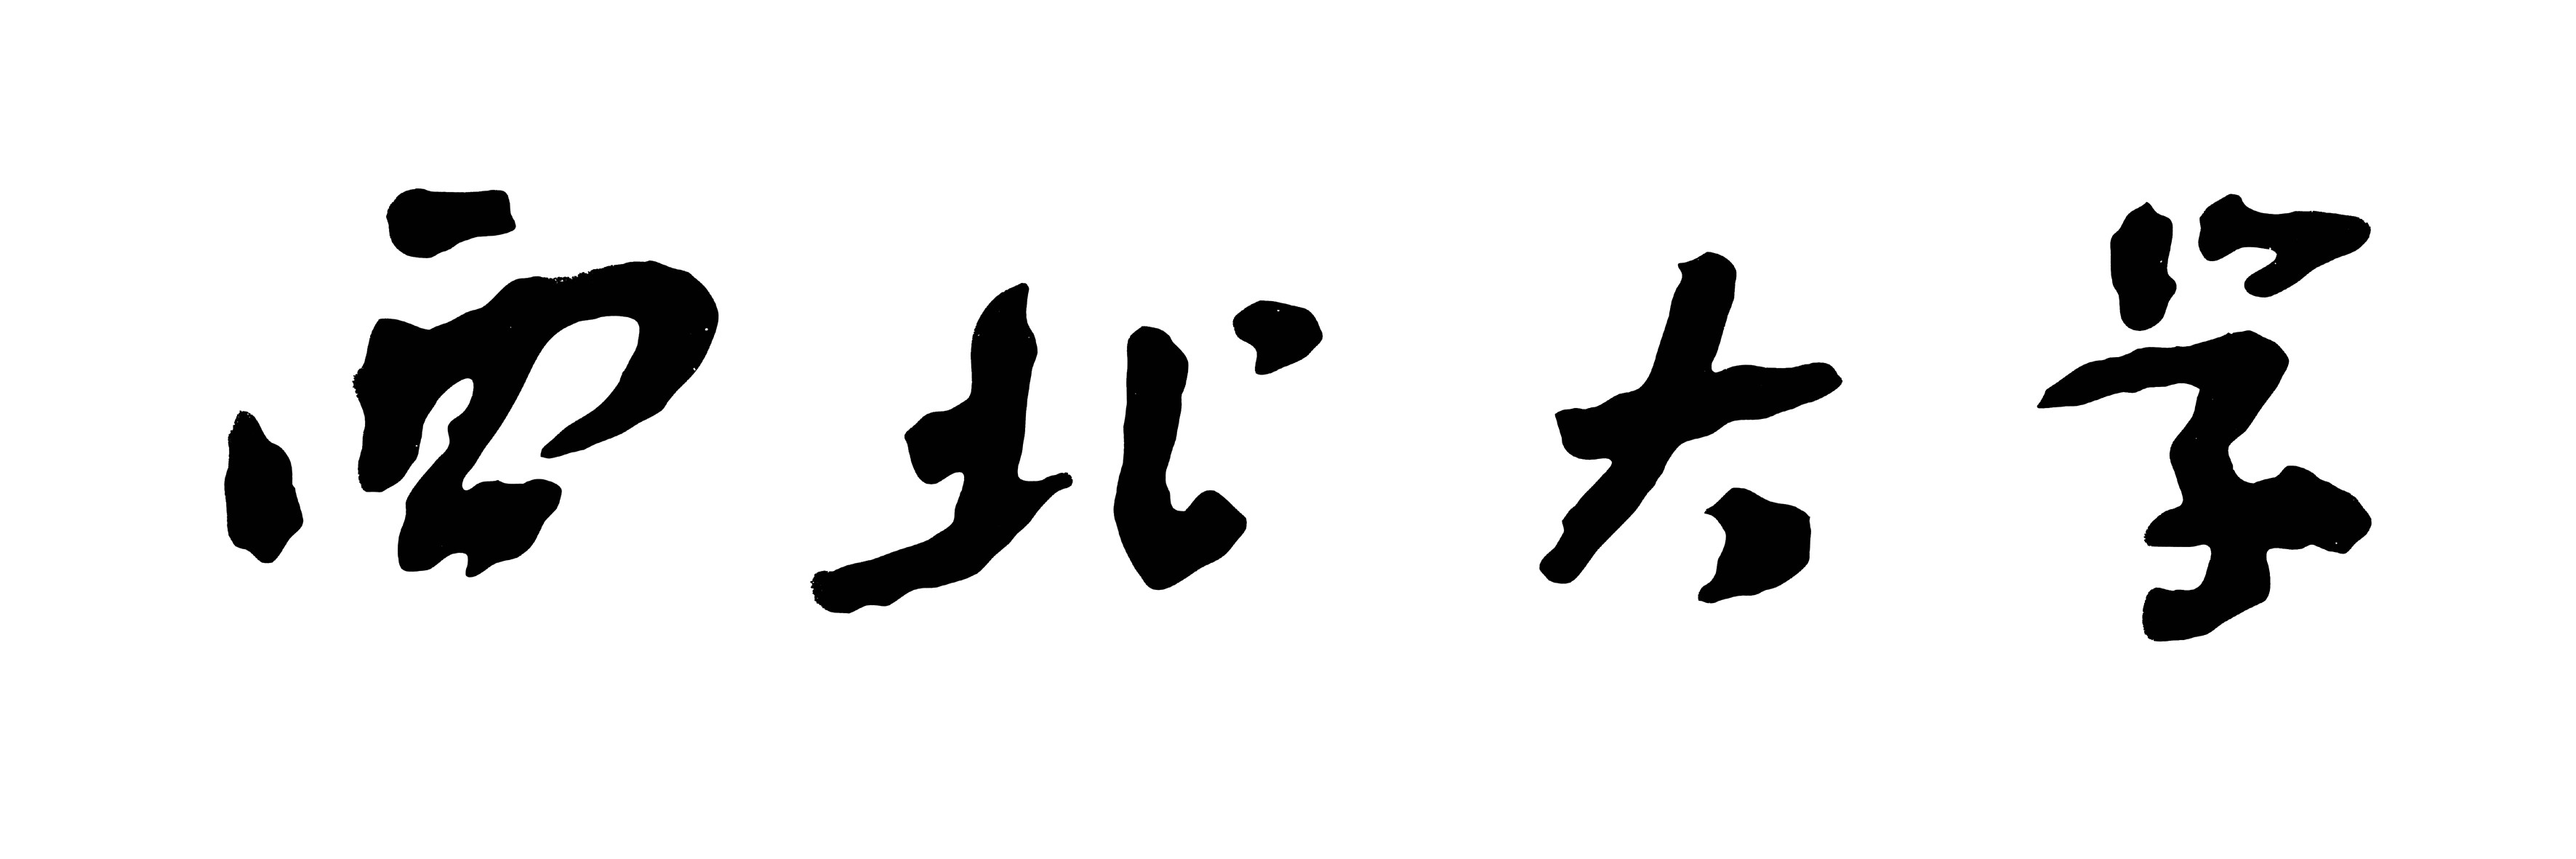
\includegraphics[width=0.6\textwidth]{nwu-name.jpg} % 插入校名
    
    \vspace{-0.1cm}
    \zihao{1}{{\kaishu\bfseries 本科毕业论文(设计)}}
    \vspace{0.5cm}

    \MakeCoverInfo
    \vspace{2cm}
    %\vfil

    % 日期
    \centering
    {\zihao{3} {\kaishu\bfseries{二〇二五年六月}}}
\end{titlepage}
\newpage
% 去除空白页的页眉和页脚
\thispagestyle{empty}  
% 插入一个空的盒子,确保页码会显示为空白页
\mbox{}  
\newpage

%正文部分前设置罗马数字
\pagenumbering{Roman}
% \newgeometry{top=2.5cm}
\begin{spacing}{2}

\section*{诚信声明}

{\zihao{4}本人郑重声明:本人所呈交的毕业论文(设计),是在导师的指导下独立进行研究所取得的成果。
毕业论文(设计)中凡引用他人已经发表或未发表的成果、数据、观点等,均已明确注明出处。
除文中已经注明引用的内容外,不包含任何其他个人或集体已经发表或在网上发表的论文。

特此声明。}
\end{spacing}
\newpage
% \restoregeometry

\section*{摘\hspace*{2em}要} % 使用 * 来避免在目录中显示摘要
这些启发式规则基于常见协议的指纹、1比特的占比以及可打印的ASCII字符的数量、比例和位置。

\vspace{28pt} 


\noindent\textbf{关键词:} 加密协议,流量分析  % 直接使用空行分隔段落

\newpage

\begin{center}
    \tableofcontents
\end{center}
\newpage

%正文部分重新设置为阿拉伯数字
\pagenumbering{arabic}  
\section{插入数学公式}
此文章是用来练习$LaTeX$的一些基本使用方法\cite{hasegawa2000plant,sunliguang2016jidi,tester2003na,zhu2002salt,mittler2002oxidative,shi2002regulation,verslues2005new,flowers1995breeding,varshney2005genomics,rengasamy2006world}。测试参考文献标注,请注意bib文件内的参考文献至少有一个被引用才可以,
先XeLaTeX编译主文件,再使用BibTeX编译一次,然后再使用XeLaTeX编译两次,一共四次\cite{sunliguang2016jidi}
\subsection{数学模式}
在行文中使用\$ ... \$ 可以插入行内公式。如$E=mc^2$.\\
在行文中使用$\backslash$begin\{equation \} ... $\backslash$end\{equation\} 可以插入行间公式。如:
\begin{equation}
E=mc^2.
\end{equation}
或者也可以写成equation*,这样就不会有编号。或者也可以使用$\backslash$[ 数学公式 $\backslash$],
这样也可以表示行间公式。\\在数学模式当中,上标为\^下标为\_并且只作用于之后的一个字符,如需要多个字符,请使用花括号括起来。
对于分式,如果要强制行内模式的分式显示为行间模式的大小,可以使用 $\backslash$dfrac, 
比如:$ \dfrac{1}{2} $
反之可以使用 $\backslash$tfrac
比如:$ \tfrac{1}{2} $,这个大小是与行间强制使用一样的
\subsection{运算符}
连加、连乘、极限、积分等大型运算符分别用$\backslash$sum, $\backslash$prod, $\backslash$lim, $\backslash$int
他们的上下标在行内公式中被压缩,以适应行高。我们可以用 $\backslash$limits 和 $\backslash$nolimits
%\quad means space
来强制显式地指定是否压缩这些上下标。例如:$ \sum_{i=1}^n i\quad \prod_{i=1}^n $
$ \sum\limits _{i=1}^n i\quad \prod\limits _{i=1}^n $
\[ \lim_{x\to0}x^2 \quad \int_a^b x^2 \mathrm{d}{x} \]
\[ \lim\nolimits _{x\to0}x^2\quad \int\nolimits_a^b x^2 \mathrm{d}{x} \]
\subsection{定界符}
在数学模式当中,可以使用大括号、中括号、小括号、单竖线、双竖线、单横线、双横线来表示定界符。
对于竖线$\vert$我们推荐使用$\backslash$vert来表示,而不是$\backslash \vert$,
把v改为大写V则表示双竖线
\subsection{省略号}
省略号用 $\backslash$dots, $\backslash$cdots, $\backslash$vdots, $\backslash$ddots 
等命令表示。$\backslash$dots 和 $\backslash$cdots 的纵向位置不同,前者一般用于有下标的序列。
\[ x_1,x_2,\dots ,x_n\quad 1,2,\cdots ,n\quad
\vdots\quad \ddots \]
\subsection{矩阵}
amsmath 的 pmatrix, bmatrix, Bmatrix, vmatrix, Vmatrix 
等环境可以在矩阵两边加上各种分隔符。
\begin{equation*}
\begin{pmatrix} a&b\\c&d \end{pmatrix} \quad
\begin{bmatrix} a&b\\c&d \end{bmatrix} \quad
\begin{Bmatrix} a&b\\c&d \end{Bmatrix} \quad
\begin{vmatrix} a&b\\c&d \end{vmatrix} \quad
\begin{Vmatrix} a&b\\c&d \end{Vmatrix}
\end{equation*}
当然也可以使用smallmatrix环境,可生成行内公式的小矩阵
$ ( \begin{smallmatrix} a&b\\c&d \end{smallmatrix} ) $
\subsection{长公式}
\subsubsection{不对齐}
无须对齐的长公式可以使用 multline 环境
\begin{multline*}
    x = a+b+c+{} \\
    d+e+f+g
\end{multline*}
\subsubsection{对齐}
需要对齐的公式,可以使用 aligned \textit{次环境}来实现,
它必须包含在数学环境之内,如果使用align则不必。插入\&表示我们希望对齐的位置,
而使用\{\}表示一个空白
\begin{equation*} 
    \begin{aligned}
        x ={}&a+b+c+ \\
             &d+e+f+g
    \end{aligned}
\end{equation*}
\subsection{公式组}
无需对齐的公式组可以使用 gather 环境,需要对齐的公式组可以使用 align 环境。
他们都带有编号,如果不需要编号可以使用带星花的版本。
\begin{gather}
    a = b+c+d \\
    (\mathrm{e}^{ax}\sin bx)^{(n)}=(a^2+b^2)^{\frac{n}{2}}\mathrm{e}^{ax}\sin (bx+n\arctan\frac{a}{b})
\end{gather}
\begin{align*}
    a &= b+c+d \\
    x &= y+z
\end{align*}
但是,如果我们是要把一个公式拆分成多行来书写,并给出一个单独的编号,就需要使用split环境。split环境需要嵌套在equation环境中,并且使用\&来标识对齐位置。
若我们需要对齐的公式组中,只有其中一行需要编号,可以用split或者gather*嵌套在equation环境中。
\begin{equation}
    \begin{split}
        a &= b+c+d \\
          &= e+f+g
    \end{split}
\end{equation}
\subsection{分段函数}
分段函数可以用cases\textit{次环境}来实现,它必须包含在数学环境之内,如公式~\ref{eq:formula}所示。
\begin{equation}
    \label{eq:formula}
    y=
    \begin{cases}
        -\sin{x}    &,x \leqslant 0 \\
        x           &,x>0
    \end{cases} 
\end{equation}
\section{插入图片和表格}
\subsection{插入图片}
利用graphicx宏包提供的$\backslash$ includegraphics命令。比如在 TeX 源文件同目录下,
有名为 a.jpg 的图片,可以用这样的方式将它插入到输出文档中:
当然也可以在导言部分使用$\backslash$gra\-phicspath\{路径\}来制定图片的搜索路径.
图片可能很大,超过了输出文件的纸张大小,或者干脆就是你自己觉得输出的效果不爽。
这时候可以用 $\backslash$includegraphics 控制序列的可选参数来控制。
比如$\backslash$includegraphics [ width = .8$\backslash$ textwidth ] \{a.jpg\}。
这样图片的宽度会被缩放至页面宽度的百分之八十,图片的总高度会按比例缩放。
其他的功能可以查看该包的文档。

\subsection{插入表格}
tabular环境提供了最简单的表格功能,用 $\backslash$hline 命令表示横线,
在列格式中用 | 表示竖线;用 \& 来分列,
用 $\backslash$$\backslash$ 来换行;
每列可以采用居左、居中、居右等横向对齐方式,分别用 l、c、r 来表示。

\begin{equation*}
    \begin{tabular}{|l|c|r|}
        \hline
       操作系统& 发行版& 编辑器\\
        \hline
       Windows & MikTeX & TexMakerX \\
        \hline
       Unix/Linux & teTeX & Kile \\
        \hline
       Mac OS & MacTeX & TeXShop \\
        \hline
       通用& TeX Live & TeXworks \\
        \hline
       \end{tabular}
\end{equation*}
有时候我们需要列出一些总结,可以使用itemize环境与$\backslash$item。而item后面可以跟一个方括号,
中括号内的东西就替换掉默认的黑点,根据需求添加序号,比如下面这个例子
\begin{itemize}
  \item 第一条        
  \item[(2)] 第二条      
\end{itemize}
或者使用下面的enumerate环境紧接方括号内label=$($ $\backslash$arabic*$)$配上自动标号
\begin{enumerate}[label=(\arabic*)]
  \item 自动标号       
\end{enumerate}
除此之外,可以使用 booktabs 宏包中的
$\backslash$toprule、$\backslash$midrule和$\backslash$bottomrule命令。
这些命令提供了更好的表格线样式,并且专门用于创建三横线表格。
\begin{equation*}
    \begin{tabular}{ccccc}
        \toprule
        姓名 & 数学 & 语文 & 英语 & 总分 \\
        \midrule
        张三 & 85 & 90 & 75 & 250 \\
        李四 & 95 & 85 & 80 & 260 \\
        王五 & 80 & 85 & 85 & 250 \\
        \bottomrule
    \end{tabular}
\end{equation*}
当然我们还可以使用插入图片的方式来进行表格的进一步控制,比如在下方添加表的名字,
可以使$\backslash$caption*\{\}的方式从而取消图片的标序,
两个表之间可以手动使用$\backslash$vspace\{2cm\}指定间隔,具体可以查看源代码
\vspace{2cm}
\begin{table}[htbp]
    \caption{公告表}
    \label{tab:Announcement}
    \centering
    \begin{tabular}{ccccc}
        \toprule
        姓名 & 数学 & 语文 & 英语 & 总分 \\
        \midrule
        张三 & 85 & 90 & 75 & 250 \\
        李四 & 95 & 85 & 80 & 260 \\
        王五 & 80 & 85 & 85 & 250 \\
        \bottomrule
    \end{tabular}
    % 使用*从而取消图片的标序
    \label{tab:grade}
\end{table}
{
    % \newcolumntype{M}[1]{>{\RaggedRight\arraybackslash}m{#1}}
    % \newcolumntype{C}[1]{>{\centering\arraybackslash}m{#1}}
\begin{table}[htbp]
  \centering
  \caption{两个医疗影像数据集的实验设置与参数对比}
  \label{tab:comparison}
  % --- 修改部分 ---
  % 将所有列都改为我们新定义的垂直居中类型
  % C{2.5cm} 用于第一列,M{4.5cm} 和 M{5cm} 用于后两列
  % \begin{tabular}{C{3.5cm} M{4.5cm} M{6cm} }
  \begin{tabular}{ 
    >{\centering\arraybackslash}m{3.5cm} |
    >{\RaggedRight\arraybackslash}m{4.5cm} | 
    >{\RaggedRight\arraybackslash}m{6cm} }
    \toprule
    % 表头不需要修改,因为 \multicolumn 会覆盖列定义
    \multicolumn{1}{c}{\textbf{维度}} & \multicolumn{2}{c}{\textbf{CovidMNIST (COVID-19 胸部 X 光分类)}} \\
    \midrule
    % 表格内容现在会自动垂直居中
    数据来源与任务 & 整合公开 COVID-19 X 光数据集, 三分 (COVID-19 / 细菌性肺炎 / 正常) & 基于 HAM10000 皮肤镜数据集, 七分类 (黑色素瘤 / 基底细胞癌等 7 类) \\
    \addlinespace 
    数据规模 & 训练集 7,000 / 验证集 1,000 / 测试集 2,000 (样本均衡度: 正常 28.6\%) & 训练集 7,010 / 验证集 1,005 / 测试集 2,000 (黑色素瘤占比 14.3\%) \\
    \addlinespace
    图像特征 & 模态: 灰度 X 光片 (28$\times$28/64$\times$64) 关键结构: 肺野、磨玻璃影 & 模态: RGB 皮肤镜图像 (28$\times$28/64$\times$64) -关键特征: 色素网络、血管模式 \\
    \addlinespace
    损失函数优化 & - 混合监督损失: 交叉熵 + KL 散度 ($\lambda$=0.5) \newline - 焦点损失: $\alpha$=0.7 (降低正常类权重) & 焦点损失: $\alpha$=0.8 (黑色素瘤权重), $\gamma$=2 (难样本放大) 聚类正则化: 强制同类样本特征距离 < 0.5 (欧氏距离约束) \\
    \addlinespace
    评价指标侧重 & 主指标: AUC-ROC (区分模糊类)、召回率 (避免漏诊) \newline 聚类指标: 轮廓系数 (验证三类分离度) & 主指标: 加权 F1 (平衡七分类)、AUC-PR (罕见病检测) \newline - 聚类指标: ARI (与病理诊断标签一致性) \\
    \bottomrule
  \end{tabular}
\end{table}


}
% 或者使用下面的enumerate环境的方法自动标号
% \begin{enumerate}[label=(\arabic*)]
%   \item         
% \end{enumerate}
\subsection{浮动体}
插图和表格通常需要占据大块空间,所以在文字处理软件中我们经常需要调整他们的位置。
figure 和 table 环境可以自动完成这样的任务;
这种自动调整位置的环境称作浮动体(float) 。我们以 figure 为例。
\begin{figure}[htbp]
    \centering
    
\includegraphics[width = .8\textwidth]{name.png}
    \caption{有图有真相}
    \label{fig:myphoto}
\end{figure}
htbp 选项用来指定插图的理想位置,
这几个字母分别代表 here, top, bottom, float page,
也就是就这里、页顶、页尾、浮动页(专门放浮动体的单独页面或分栏)。
$\backslash$centering 用来使插图居中;
$\backslash$caption 命令设置插图标题,
LaTeX会自动给浮动体的标题加上编号。注意$\backslash$label 应该放在标题命令之后。
但是实际上浮动图片的问题并非想象中的简单,这里碍于时间限制暂时写到这里。
补充一点,如果想让两个图片同行显示可以使用$\backslash$subfigure,效果如下
\begin{figure}[htbp]
    \centering
    \begin{subfigure}[b]{0.45\textwidth}
        
\includegraphics[width=\textwidth]{name.png}
        % \caption{}
        \label{fig:image1}
    \end{subfigure}
    \hfill
    \begin{subfigure}[b]{0.45\textwidth}
        
\includegraphics[width=\textwidth]{name.png}
        % \caption{}
        \label{fig:image2}
    \end{subfigure}
    \caption{有图有真相2}
    \label{fig:twosubfigs004}
\end{figure}
\section{版面设置}
\subsection{行间距}
\noindent 可以使用$\backslash$noindent指定第一行不缩进。
我们可以通过 setspace 宏包提供的命令来调整行间距。
比如在导言区添加
$\backslash$usepackage\{setspace\}
$\backslash$onehalfspacing,可以将行距设置为字号的 1.5 倍:
请注意用词的差别:行距是字号的 1.5 倍;1.5 倍行距。
事实上,这不是设置 1.5 倍行距的正确方法。
\subsection{段间距}
我们可以通过修改长度$\backslash$parskip 的值来调整段间距。在导言区添加
$\backslash$addtolength\{par\-skip\}\{.4em\}
则可以在原有的基础上,增加段间距 0.4em。如果需要减小段间距,只需将该数值改为负值即可。
\subsection{字体}
在数学模式中,可以使用$\backslash$textit\{\}, $\backslash$textbf\{\}, 
$\backslash$textsf\{\}, $\backslash$texttt\{\}来表示字体。
\newpage
\addcontentsline{toc}{section}{参考文献}

% .bib 文件名(不带扩展名)
\bibliography{bib/reference}
\bibliographystyle{gbt7714-2005-numerical} 

\end{document}